%%%%             %%%%
%%%% ADICIONAL 1 %%%%
%%%%             %%%%

\chapter{Material adicional}
\label{chap:adicional-1}

\lettrine{E}{n} este apéndice se presentan imágenes de los documentos tratados en el trabajo. También se muestran los directorios y ficheros de código fuente creados. En último lugar se puede encontrar el manual de instalación y uso del software.

% TODO valorar si añadir capturas de 
% TODO - formato de un PDF

\section{Ejemplos de los documentos tratados}

% TODO añadir imágenes de los documentos tratados

\section{Directorios y código fuente del proyecto}

\begin{figure}[hp!]
    \centering
    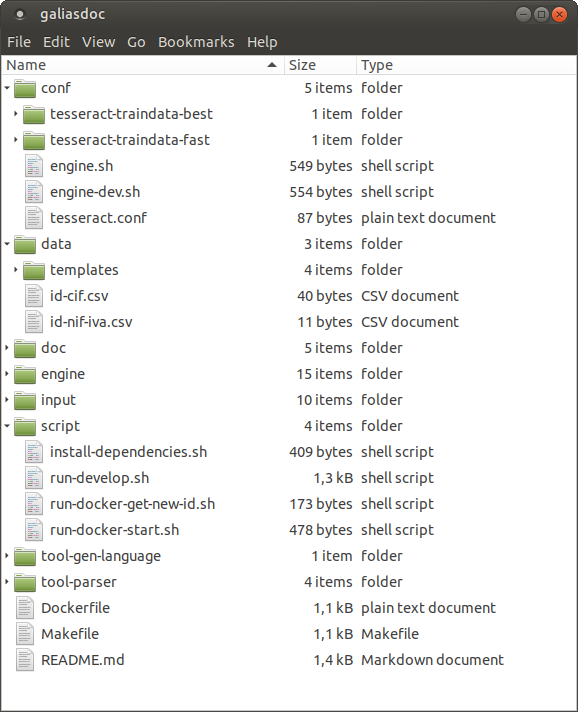
\includegraphics[width=0.8\textwidth]{imaxes/adicional-1/estructura-general.png}
    \caption{Directorios del proyecto}
    \label{fig:directorios-proyecto}
\end{figure}

\begin{figure}[hp!]
    \centering
    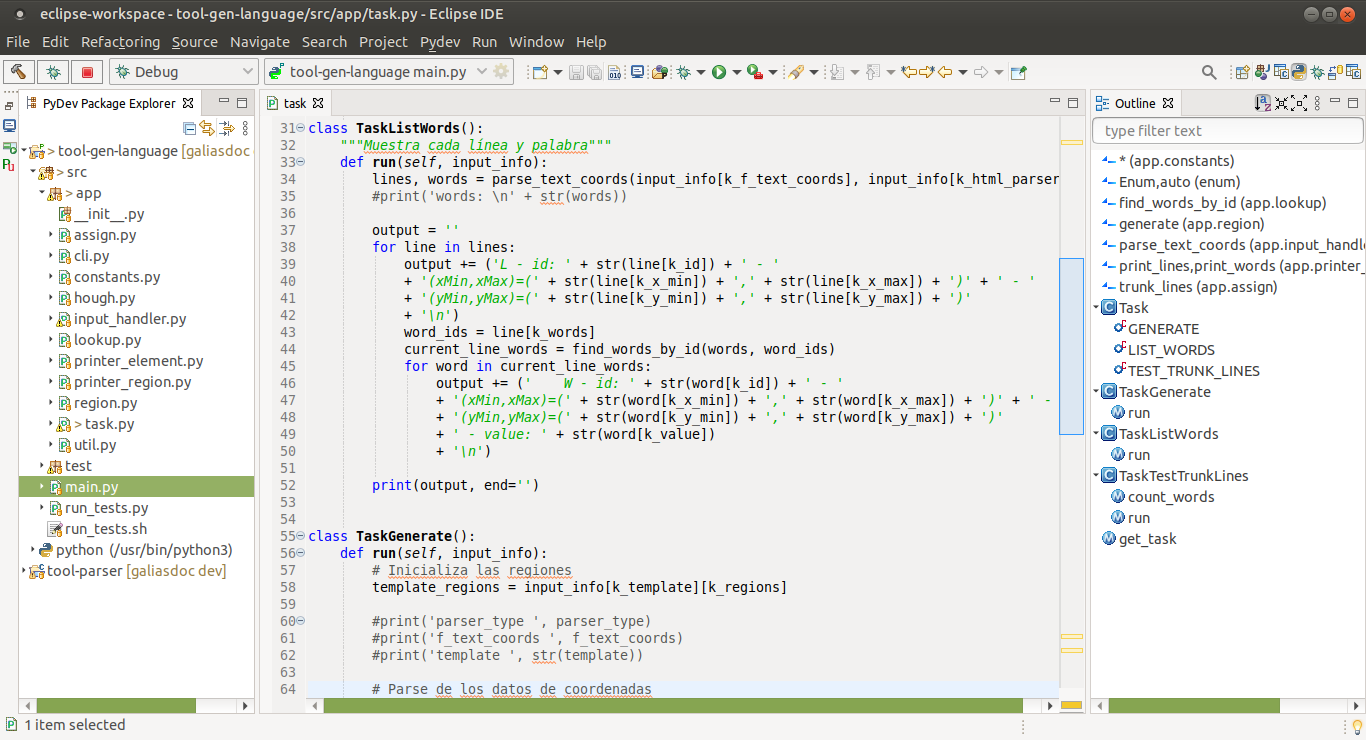
\includegraphics[angle=90,height=1.6\textwidth]{imaxes/adicional-1/tool-gen-language-pydev.png}
    \caption{Proyecto del generador de código intermedio en Pydev}
    \label{fig:tool-gen-language-pydev}
\end{figure}


\noindent\begin{minipage}{.45\textwidth}
\begin{lstlisting}[caption=Scripts del engine,frame=tlrb]{Name}
tool-gen-language/
  engine/
    extract-images.sh
    extract-text-coords.sh
    extract-text.sh
    fix-page-numbers.sh
    generate-images-for-text-based.sh
    generate-json.sh
    get-job-id.sh
    identify-grep.sh
    image-apply-blur.sh
    image-apply-ocr.sh
    image-apply-unskew.sh
    populate-result.sh
    run.sh
    split-text-from-image.sh
    unpack.sh
\end{lstlisting}
\end{minipage}\hfill
\begin{minipage}{.45\textwidth}
\begin{lstlisting}[caption=Fuentes del procesador de lenguaje intermedio,frame=tlrb]{Name}
tool-parser/
    Makefile
    lib/
        cJSON.c
        cJSON.h
        lista.c
        lista.h
        reg-exp.c
        reg-exp.h
        strbuf.c
        strbuf.h
        util.c
        util.h
    main/
        app-conf.h
        bison-epilogue.c
        bison-epilogue.h
        bison-prologue.c
        bison-prologue.h
        flex-prologue.c
        flex-prologue.h
        gen-amount.c
        gen-amount.h
        gen.c
        gen.h
        global-vars.h
        main.c
        main.h
        types.h
    plugin/
        A48941488.l
        A48941488.y
        B15035801.l
        B15035801.y
        B83834747.l
        B83834747.y
        IE6364992H.l
        IE6364992H.y
\end{lstlisting}
\end{minipage}

\section{Instalación de software}

La instalación completa desde el código fuente implica la descarga del contenido presente en el repositorio git.

En esta sección se asume que se utilizará una distribución Ubuntu 18.04 igual a la empleada durante el desarrollo. Para la correcta compilación y ejecución es necesario que varias aplicaciones y librerías estén disponibles en el sistema. En el caso de las nuevas versiones de Ubuntu, la lista de paquetes a instalar no presentará diferencias pero si se utiliza Fedora u otras será necesario averiguar que paquetes contienen el software utilizado e instalarlos.

Se pueden distinguir dos escenarios distintos. Los requisitos necesarios para compilar los fuentes y aquellos imprescindibles únicamente para ejecutar la aplicación. Para el primer caso se debe utilizar el comando mostrado en \ref{lst:requisitos-para-compilacion}. El paquete \verb|build-essential| instala la mayor parte de las aplicaciones como el compilador de C y Make.

\begin{lstlisting}[language=bash,caption={Dependencias para la compilación},label=lst:requisitos-para-compilacion]
sudo apt-get build-essential libpcre2-dev bison flex
\end{lstlisting}

En el caso de tener ya la aplicación compilada y empaquetada, será necesarios instalar los componentes para la ejecución, como Tesseract, el software de OCR. La orden del listado \ref{lst:requisitos-para-ejecucion} instalará estos requisitos.

\begin{lstlisting}[language=bash,caption={Dependencias para la ejecución},label=lst:requisitos-para-ejecucion]
sudo apt-get install unzip poppler-utils mediainfo tesseract-ocr tesseract-ocr-spa jq python3-opencv jq bc
\end{lstlisting}

De manera opcional, pero recomendable, se puede utilizar un PPA específico para obtener una versión actualizada de Tesseract. Un PPA en el entorno Ubutnu, es un repositorio personal, en este caso mantenido por Alexander Pozdnyakov \footnote{\url{https://launchpad.net/~alex-p/+archive/ubuntu/tesseract-ocr}}. La activación de este repositorio debe hacerse previamente a la instalación del software. En necesario ejecutar los comandos del listado \ref{lst:activar-ppa-tesseract}.

\begin{lstlisting}[language=bash,caption={Activar PPA},label=lst:activar-ppa-tesseract]
sudo add-apt-repository ppa:alex-p/tesseract-ocr
sudo apt-get update
\end{lstlisting}

No se ahondará en el uso del software ya que ha sido explicado en detalle en el capítulo \ref{chap:implemetación}.
